\subsection{Ballerkennung}

\label{sec:balldetection}
Die Ballerkennung läuft in einen eigenen Thread im Client, da sie und
die Fahrschleife des Roboters sich gegenseitig blockieren
würden. Dabei greift sie auf das Kamerabild einer Logitech Webcam Pro 9000
zurück. Nach Initialisierung der Ballerkennung
werden folgende Schritte durchgeführt, bis der Ball gefunden oder die
Suche abgebrochen wurde:

\begin{nofloat}{figure}
\centering
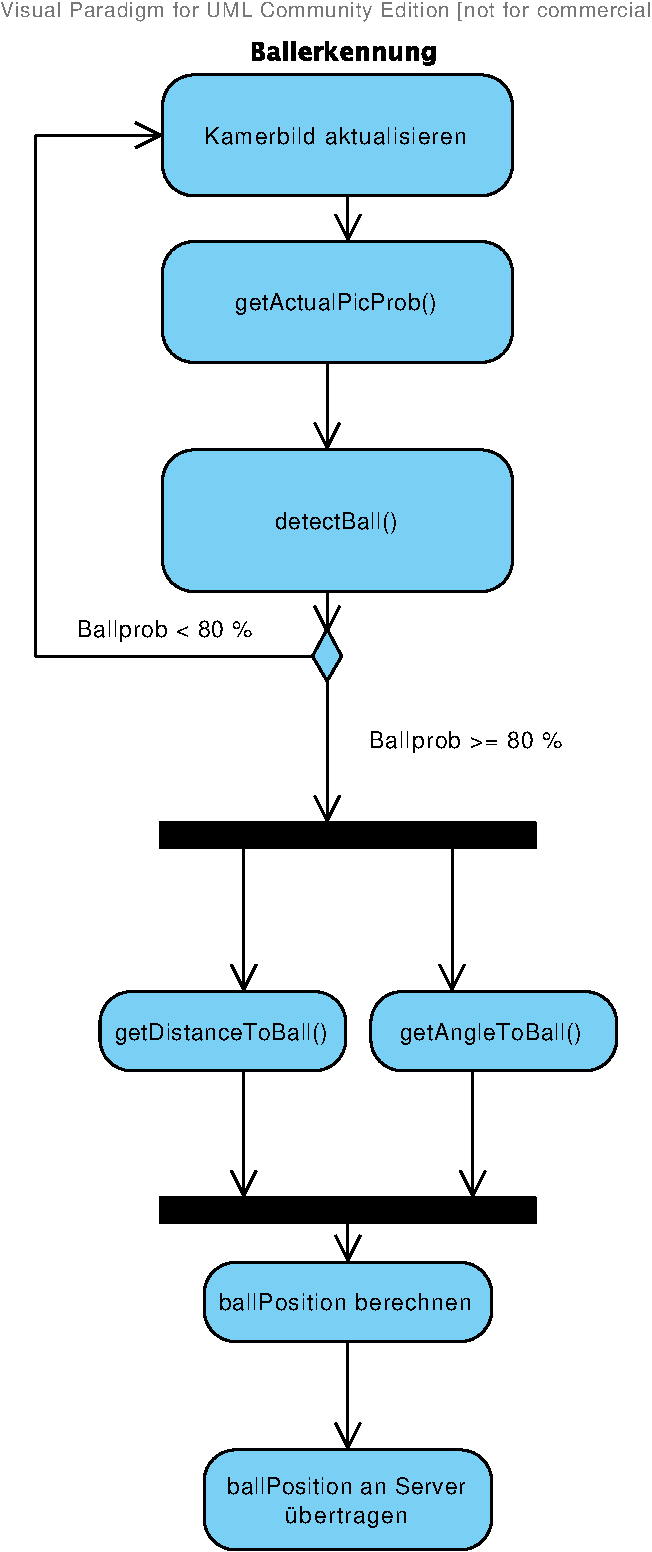
\includegraphics[width=0.5\linewidth]{bilder/balldetect_uml}
  \caption{Ablauf der Ballerkennung}
\end{nofloat}
%\begin{enumerate}
%\item Aktualisieren des aktuellen Kamerabildes
%\item Aufruf der Erkennungsmethode der Balldetection
%  \lstinline|detectBall()|. 
%\item Abfrage, ob der Ball erkannt wurde mit der Methode
%  \lstinline|getActualPicProb()|. Liefert diese eine
%  Wahrscheinlichkeit zurück, die größer als 80 \% ist, ist die Suche
%  beendet und die Koordinaten des Balls werden wie folgt bestimmt:
%  \begin{enumerate}
Die Berechnung der Ballposition arbeitet dabei wie folgt:\\
%\begin{itemize}
% \item
 Mit den Methode \lstinline|getDistanceToBall()| und
    \lstinline|getAngleToBall()| wird die Entfernung (in mm) und der Winkel
    zum Ball (in Grad von der Mitte des Bildes aus ($0^\circ$), links positiv, rechts
		negativ) abgerufen. 
%              \item 
Aus den Ergebnissen wird zusammen mit der aktuellen Position des Roboters
    die Ballposition für die Anzeige auf der Karte des Servers bestimmt, dazu wird zuerst der Ausrichtungsvektor des
		Roboters um den Winkel zum Ball gedreht.
             % \item 
Dann wird die Entfernung zum Ball ermittelt, da diese in mm ist, muss
die Entfernung in px (auf der Serverkarte) umgerechnet werden. Dazu dient der Wert
pixelPerMm aus der Konfiguration, welcher die Auflösung der Karte in px/mm angibt. Um nun die Ballposition zu
	erhalten, wird der gedrehte Ausrichtungsvektor (ein Einheitsvektor) mit
		pixelPerMm $\cdot$ Entfernung zum Ball skalar multipliziert und zum aktuellen
		Positionsvektor addiert.
%  \item 
Danach wird die gefundene Position zum Server übertragen.
\\\\
Wie bereits erwähnt greifen wir bei der Ballerkennung auf die
Bachelorarbeit von Tobias Breuer zurück. Dadurch konnten wir einfach
die API der von ihm entwickelten Software nutzen, ohne uns selber mit
den Details der Ballerkennung beschäftigen zu müssen. Sie verfolgt
folgenden Ansatz: Im Kamerabild wird nach roten Pigmenten
gesucht. Erreichen diese eine gewisse Anzahl, sucht die Software nach
kreisförmigen Objekten, die diese Pigmente enthalten. Je nachdem,
wie weit diese Kriterien erfüllt sind, berechnet die Software eine
Wahrscheinlichkeit, ob sich im aktuellen Bild ein Ball befindet und
die Entfernung und den Winkel zum vermuteten Ball. Um vernünftige
Werte zu erhalten ist es unabdingbar, die Software vorher zu
kalibrieren\footnote{Die genaue Vorgehensweise wird im Abschnitt
\ref{cha:nutzung} Nutzung ab Seite \pageref{cha:nutzung} beschrieben}.  Nichts
destotrotz kann es zu False-Positives
kommen. Näheres zu den  Ursachen von
False Positives finden sich im Abschnitt \ref{cha:evaluation} ab Seite \pageref{cha:evaluation}.
%%% Local Variables: 
%%% mode: latex
%%% TeX-master: "template"
%%% End: 
